\chapter{Parsimonious Vole grammar}
\label{ch:the-grammar}

Now that the main theoretical foundations have been covered, I describe the structure of grammatical units and system networks adopted in this thesis and implemented in the Parsimonious Vole parser. Some of them are from the Sydney and others from the Cardiff grammars. There are many common parts but also differences in parts of their paradigmatic and syntagmatic descriptions. %Just like in the previous chapter I base my discussion on pragmatic grounds.

First I discuss the structural differences between main units in the Sydney and the Cardiff grammars: the clause, the verbal group, nominal group, the adjectival and adverbial groups. Then, I focus on two important system networks: TRANSITIVITY  and MOOD. The first is adopted from the Cardiff grammar and the second belongs to the Sydney grammar.

\section{Grammatical units}
\label{sec:discussion-unit-classes}

%I turn now to discuss the structure of the units implemented in the Parsimonious Vole parser. I provide arguments and reasoning for choosing one over the other unit structure. 
The general principle for selection is that some unit structures are closer to traditional syntactic analysis and so possible to connect the elements of the Dependency grammar. There are some units in both Sydney and Cardiff grammars that fit this purpose and some others that are semantically grounded and are more difficult to capture in structural variance, requiring additional lexical-semantic resources. This section discusses choices made for the current work.

%For the reasons of limited space I skipped introducing the Sydney and Cardiff grammars and in turn assume that the reader is familiar with the details fo both of them. And for a general overview of the unit structure in each of the grammars please refer to Appendix \ref{ch:syntax-overview}. 
%Nevertheless, as it is a parallel contrasting discussion, even if the reader is familiar with one grammar only I hope it becomes clear how does certain phenomena are dealt with in the other one. 

\subsection{Verbal group and clause boundaries}
\label{sec:verbal-grpoup-and-clause-division}
In the Sydney Grammar the verbal group is described as an expansion of a verb just like the nominal group is the expansion of the noun \citep[396]{Halliday2013}. There are certainly words that are closely related and syntactically dependent on the verb all together forming a unit that functions as a whole. For example the auxiliary verbs, adverbs or the negation particles are words that are directly linked to a lexical verb. The verb group functions as Finite + Predicator elements of the clause in Mood structure and as Process in Transitivity structure. 

In the Cardiff Grammar the verb group is dissolved, moving the Main Verb to the pivotal element of the Clause unit. All the elements that form clause structure and those that form verb group structure are brought together to the same level as elements of a clause. The clause structure in the Cardiff Grammar comprises elements with clause related functions (like Subject, Adjunct, Complement etc.) and other elements with Main Verb related functions (Auxiliary, Negation particle, Finite operator etc.).

Regarded from the Hallidayan rank scale perspective, merging the elements of the verb group into clause structure is not permitted because the units are at different ranks. However this is not a problem for the relaxed rank scale version presented in Section \ref{sec:rank-system}. The reason for adopting such an approach is best illustrated via complex verb groups with more than one non-auxiliary verb as in Examples \ref{ex:complex-verb-groups1}--\ref{ex:complex-verb-groups3}. 

I begin by addressing the impact of this merger on (a) the clause structure (b) the clause boundaries and (c) the semantic role distribution within the clause.

\begin{exe}
	\ex\label{ex:complex-verb-groups1}
	(The commission \textit{started to investigate} two cases of over-fishing in Norway.)  
	\ex\label{ex:complex-verb-groups2}
	(The commission \textit{started} (\textit{to investigate} two cases of over-fishing in Norway.))
	\ex\label{ex:complex-verb-groups3}
	(The commission \textit{started} (\textit{to finish} (\textit{investigating} two cases of over-fishing in Norway.)))
\end{exe}

%Then answers to the above questions boil down to whether we allow for more than one lexical verb per predicate or not. 
In the Sydney Grammar ``started to investigate'' (in Example \ref{ex:complex-verb-groups1}) is considered a single predicate of investigation which has specified the aspect of event incipiency despite the fact that there are two lexical verbs within the same verbal group. The ``starting'' doesn't constitute any kind of process in semantic terms but rather specifies aspectual information about the investigation process. This is argued by looking at the conditions on participants and it is equivalent in a formal approach to looking at where the selection restrictions for complements come from. The boundaries of the clause governed by this predicate stretch to the entire sentence.

Semantically it is a sound approach. Despite the presence of two lexical verbs there is only one event. However, allowing such compositions leads to unwanted syntactic analysis for multiple lexical verb cases in examples such as \ref{ex:complex-verb-groups3}. To solve this kind of problem Fawcett dismisses verb groups and merges their elements within clause structure. He proposes the syntactically elegant principle of \textit{one main verb per clause} \citep{Fawcett2008}. Applying this principle to the same sentence yields a structure of two clauses illustrated in example \ref{ex:complex-verb-groups2} where the main clause is governed by the verb ``to start'' and the embedded one by the verb ``to investigate''. Note the conflict of ``one main verb per clause'' with Halliday's principle that only whole units form the constituency of others (the (c) principle of rank scale described in Section \ref{sec:rank-system}). So allowing incomplete groups into the constituency structure would breach the entire idea of unit based constituency. 

Semantically the clause in SFL is a description of an event or situation as a figure with a process, participants and eventually circumstances where the process is realised through a lexical verb. Looking back to our examples, the question is then does the verb ``to start'' really describe a process or merely an aspect of it? Halliday treats such verbs as aspectual and when co-occurring with other lexical verbs they are considered to form a single predicate. Accommodating Fawcett's stance, mentioned above and contradicting Halliday's approach, requires weakening the semantic requirement and allowing aspectual verbs to form clauses that contribute \textit{aspectually or modally} to the embedded ones. I mention also the modal contribution because some verbs like \textit{want, wish, hope} and others behave syntactically like the aspectual ones. Moreover, Fawcett introduces into the Cardiff Grammar Transitivity network an \textit{influential} process type including all categories of meanings that semantically function as process modifiers: tentative, failing, starting, ending etc.

I adopt here Fawcett's ``one main verb per clause'' principle, which as a consequence changes the way clauses are partitioned, leads to abolition of the verbal group and introduces the ``influential'' process type. Next I discuss the impact of this verb group abolition on the structure of clause units. 

\subsection{Clause}
\label{sec:cardiff-clause}
It is commonly agreed in linguistic communities that the unit of the clause is one of the core elements in human language. 
%It is considered the syntactic unit that expresses semantic units of a situation referring to a potentially rich array of meanings. The clause structure has been studied for long time and 
The main clause constituents are roughly the same in SFL as the ones in traditional grammar \citep{Quirk1985}, transformational grammar \citep{Chomsky57} and indirectly in dependency grammar \citep{Hudson2010}.

%As mentioned before in Definition \ref{def:structure} the elements of a structure are defined in terms of their function contributing to the formation of the whole unit.
I adopt the Cardiff Grammar clause structure where \textit{Main Verb} is the pivotal element of the unit. The clause is formed of the \textit{Subject}, \textit{Finite}, \textit{Main Verb}, up to two \textit{Complements} and a various number of \textit{Adjuncts}. All the elements that in the Sydney grammar are part of the verbal group, such as Auxiliary Verbs, Main Verb Extensions, Negators etc. are considered part of the clause structure. For a complete list see Appendix \ref{ch:syntax-overview}.

\begin{exe}
	\ex\label{ex:elipted-clause} They were in the bar, \textit{Dave in the restroom and Sarah by the bar}.
\end{exe}
%In current work the Cardiff Grammar clause structure is adopted where the \textit{Main Verb} is the pivotal element. 
Although there is no element that is obligatorily realised in English, I consider in the current work that every non-auxiliary lexical verb is a Main Verb and thus flags presence of a clause unit. 
There are clauses, in SFL, without a main verb, such as minor clauses (exclamations, calls, greetings and alarms) that occur in conversational contexts and elliptical clauses \citet{Halliday2013} such as the one in Example \ref{ex:elipted-clause}, none of which are covered in the present work.

%%TODO insert the complete list as done for nominal group below

%\todo*{}{TODO continue, maybe mention about the clause complexing}
%SFG accounts for how clauses form nexuses of tactic relations (see Definition \ref{def:taxis}).


\subsection{Nominal Group}
\label{sec:nominal-group}

The nominal group expresses things, classes of things or a selection of instances in a class. This section argues for adoption of the Sydney grammar noun group structure with a slight modification. The elements of the nominal group can be filled, in addition to word units, by group units as well. This possibility is opened by the rank scale relaxation (Section \ref{sec:rank-system}) and the Cardiff embedding principle (Definition \ref{def:embedding}). Cardiff's nominal units would be more difficult to process because of their semantic nature and are left out of the current implementation for further work. Nonetheless, I argue below for working towards semantic and syntactic heads in two steps: first create the structure with the syntactic one (the Head) and then derive the semantic one (the Thing), eventually arriving at the Cardiff nominal structure.

\begin{table}[!ht]
    \centering
	\begin{tabular}{|c|c|c|c|c|c|}
		\hline
		\textit{those} & \textit{two} & \textit{old} & \textit{electric} & \textit{trains} & \textit{from Luxembourg} \\ \hline
		\multicolumn{4}{|c|}{Pre-Modifier}                               & Head            & Post-Modifier            \\ \hline
		Deictic        & Numerative   & Epithet      & Classifier        & Thing           & Qualifyier               \\ \hline
		determiner     & numeral      & adjective    & adjective         & noun            & prepositional phrase     \\ \hline
	\end{tabular}
	\caption{An example of a nominal group in the Sydney Grammar \citep[264]{Halliday2013}}
	\label{tab:example-ng}
\end{table}

In  Table \ref{tab:example-ng} an example analysis is presented of the nominal group proposed in the Sydney grammar \citep[364--369]{Halliday2013}. The Sydney nominal group is constituted by a head nominal item modified by descriptors or selectors such as: \textit{Deictic}, \textit{Numerative}, \textit{Epithet}, \textit{Classifier}, \textit{Thing} and \textit{Qualifier}. Each element has a fairly stable correspondence to the word classes expected to be expounded by lexical items. Table \ref{tab:function-pos-mapping} presents the mappings between the elements of nominal group and the word classes. 

\begin{table}[!ht]
        \centering
	\begin{tabulary}{0.9\linewidth}{|C|C|}
		\hline
		\textbf{Experiential function in noun group} & \textbf{class (of word or unit)} \\ \hline
		Deictic                             & determiner, predeterminer, pronoun, adjective \\ \hline
		Numerative                          & numeral(ordinal or cardinal) \\ \hline
		Epithet                             & adjective \\ \hline
		Classifier                          & adjective, noun \\ \hline
		Thing                               & noun                         \\ \hline
		Qualifier                           & prepositional phrase, clause \\ \hline
	\end{tabulary}
	\caption{Mapping of noun group elements to classes \citep[379]{Halliday2013}}
	\label{tab:function-pos-mapping}
\end{table}

Inspired from the Cardiff grammar, in addition to word classes the elements of the nominal group can also be filled by the group classes corresponding to each word class above. This way the Numerative, in addition to words, can be filled by a noun group, Epithet by an adjectival group, Classifier by an adjective or noun group and finally each of the elements can be filled by a coordination group as discussed in Section \ref{sec:coordination}.

%There is little variation in how these functions are linked to the word classes. However the variation is not provided in the Sydney Grammar as it is in Cardiff Grammar. The latter provides data driven filling probabilities for each functional element to a set of possible unit classes \citep{Fawcett2000}.

The elements in the Cardiff Grammar differ from those of the Sydney Grammar. Table \ref{tab:carfiff-ng} exemplifies a noun group analysed with the Cardiff Grammar covering all the possible elements. Table \ref{tab:cg-mappings} provides a legend for the Cardiff Grammar acronyms along with mappings to unit and word classes that can fill each element.

    \begin{table}[!ht]
	\resizebox{\linewidth}{!}{
		\begin{tabular}{|c|c|c|c|c|c|c|c|c|c|c|c|c|c|c|}
			\hline
			\textit{or} & \textit{a photo} & \textit{of} & \textit{part} & \textit{of} & \textit{one} & \textit{of} & \textit{the best} & \textit{of} & \textit{the} & \textit{fine} & \textit{new} & \textit{taxis} & \textit{in Kew} & \textit{,} \\ \hline
			\multicolumn{12}{|c|}{pre-modifiers} & head & \multicolumn{2}{c|}{post-modifiers} \\ \hline
			\& & rd & v & pd & v & qd & v & sd or od & v & dd & m & m & h & q & e \\ \hline
		\end{tabular}}
		\caption{The example of a nominal group in Cardiff Grammar}
		\label{tab:carfiff-ng}
	\end{table}
	%
	\begin{table}[!ht]
		\begin{tabulary}{\textwidth}{|C|C|C|}
			\hline
			\textbf{symbol} & \textbf{function meaning} & \textbf{class (of word or unit)} \\ \hline
			rd & representational determiner & noun, noun group \\ \hline
			v & selector ``of'' & preposition \\ \hline
			pd & partitive determiner & noun, noun group \\ \hline
			fd & fractional determiner & noun, noun group, quantity group \\ \hline
			qd & quantifying determiner & noun, noun group, quantity group \\ \hline
			sd & superlative determiner & noun, noun group, quality group, quantity group \\ \hline
			od & ordinative determiner & noun, noun group, quality group \\ \hline
			td & tipic determiner & noun, noun group \\ \hline
			dd & deictic determiner & determiner, pronoun, genitive cluster \\ \hline
			m & modifier & adjective, noun, quality group, genitive cluster \\ \hline
			h & head & noun, genitive cluster \\ \hline
			q & qualifier & prepositional phrase, clause \\ \hline
			\& & linker & conjunction \\ \hline
			e & ender & punctuation mark \\ \hline
		\end{tabulary}
		\caption{The mapping of noun group elements to classes in Cardiff grammar}
		\label{tab:cg-mappings}
	\end{table}
	%
	
The elements in the Cardiff Grammar are based on semantic criteria supported by lexical and syntactic choices. Consequently some elements cannot be derived on solely syntactic criteria, requiring semantically motivated lexical resources. The challenging semantically bound elements from Cardiff grammar are the following determiners \textit{Representational, Partitive, Fractional, Superlative, Typic Determiners}, while the rest of the elements: \textit{Head, Qualifier, Selector, Modifier and Deictic, Ordinative and Quantifying Determiners} can be determined solely on the syntactic criteria. The latter correspond fairly well to the Sydney version of the nominal group, which is adopted in the present work. In addition the relaxed rank scale discussed in Section \ref{sec:rank-system} permits replacing the nominal group sub-structures from the Sydney grammar with embedded units just like in the Cardiff grammar simplifying the syntactic structures.
	
	%3. introduction of negation element, linker, punctuation
	%``No'' as determiner. negative pronoun noone.
	%\citep[62,109,185]{Quirk1985}, \citep[365--374]{Halliday2013}, 
	%
	%The negation element is in Cardiff Grammar in clause structure so that it is separated from the finite. It's adoption in noun structure might or might not be a good idea. It is useful for complex groups. 
	%
	%\begin{exe}
	%\ex \label{ex:example-of-no}
	%No breathing man or animal can escape that forest alive.
	%\end{exe} 
	
Another simplification is renouncing distinction between the Head and Thing \citep[390--396]{Halliday2013} discussed in Section \ref{sec:heads}. Thus if the logical Head of the nominal group is a noun then it is labelled as the Thing leaving the semantic discernment as a secondary process and out of the current scope. Otherwise, in cases of nominal groups without the Thing element, if the Head is a pronoun (other than personal), numeral or adjective (mainly superlatives), then it functions as Deictic, Numerative or Epithet. So, as will be described in Chapter \ref{ch:parsing-algorithm}, I propose to parse nominal groups in two steps: first determine the main constituting chunks and assign functions to the unambiguous ones and, second, perform a semantically driven evaluation for the less certain units. 
%However, in the present work the second step has not been covered. 
	
%	\todo*{probably remove: discussion of Head/Thing and Cardiff Grammar determiners distinction}{
Next I explain this two step process, using for illustration cases when the Thing is present but is different from the Head as in examples \ref{ex:dectic-ngs}--\ref{ex:dectic-ngs2}.

\begin{exe}
    \ex \label{ex:dectic-ngs} (a cup) of (tea)
    \ex \label{ex:dectic-ngs1}(some) of (those youngsters)
    \ex \label{ex:dectic-ngs2}(another one) of (those periodic eruptions)
\end{exe}

These nominal groups can be analysed in two ways. They are either about the ``cup'', ``some'' or ``another one'', leading to a structure where the first noun is the head succeeded by a prepositional phrase Qualifier, or about ``tea'', ``youngsters'' and ``eruptions'', where the second noun is the head and so adopting a structure with complex determiners.

Table \ref{tab:exmaple-analisys-parsing-syn-sem-heads} shows on the first row an analysis with syntactic head, i.e. the Head defined in the Sydney grammar, and on the second row an analysis with semantic head, i.e. the Head defined in the Cardiff grammar that also coincides with the Thing from the Sydney grammar.

At a particular level of structural embedding, the syntactic Head is always the first noun in the nominal group. In the semantic evaluation phase special attention is given to Qualifiers filled by prepositional phrases starting with preposition ``of'' and whether the nominal group may function as qualifying, quantifying, ordination or other type of determiner. 

The Cardiff Grammar weakens the assumption that every prepositional phrase acts as Qualifier in a nominal group and treat the preposition ``of'' as a special case. This preposition is allowed to act not as the element introducing a prepositional phrase but as a end mark of a determiner-like selector. When such a selector is present the preceding noun group functions as a Determiner (of some sort) to the noun or nominal group as can be seen in Table \ref{tab:exmaple-analisys-parsing-syn-sem-heads}. 

% As mentioned earlier, I adopt a here the Sydney approach to nominal group structure. But this analisys 
The nominal groups that contain a prepositional phrase Qualifier introduced by the preposition ``of'' receive a special attention because they may qualify to the special case explained earlier. If the above condition is satisfied then, in a second phase of nominal group analysis aiming at the semantic evaluation, the prepositional phrase Qualifier is disassembled, the preposition ``of'' is ascribed a Selector function of the parent nominal group, being transferred upwards in the structure, and the preceding nominal group (syntactically headed) becomes one of the determiners. This approach shifts the noun group head into the position of a semantically based Thing and evades the discrepancy problem between them. This 

\begin{table}[!ht]
    \centering
    \begin{tabular}{c|c|c|c|c|}
    \cline{2-5}
     & \textit{a} & \textit{cup} & \textit{of} & tea \\ \hline
    \multicolumn{1}{|c|}{1st step} & Determiner & Head & \multicolumn{2}{c|}{Qualifier} \\ \hline
    \multicolumn{1}{|c|}{2nd step} & \multicolumn{2}{c|}{Quantifying Determiner} & Selector & Head/Thing \\ \hline
    \end{tabular}
    \caption{Example analysis with syntactic and semantic heads performed in two steps}
    \label{tab:exmaple-analisys-parsing-syn-sem-heads}
\end{table}

The above explanation is not a straightforward solution. The distinction between cases when the proposition ``of'' introduces a Qualifier or ends a Selector/Deictic requires a lexical-semantic informed decision answering the question ``what is the Thing that this nominal group is about?''. And there is a lot of space for variations in the syntactic structure. For example in example \ref{ex:of-qualifiers} (where Head/Thing is marked in italic) the preposition ``of'' introduces Qualifiers.
 
 \begin{exe}
    \ex \label{ex:of-qualifiers}He was the \textit{confidant} of the prime minister.
    \ex It was the \textit{clash} of two cultures.
\end{exe}

This section has discussed the problem of semantic and syntactic heads (started in Section \ref{sec:heads}) applied to nominal groups in particular and how to approach parsing them. I conclude that it is fairly unambiguous and straightforward to determine the structure of nominal groups according to the Sydney grammar yielding a syntactically based structure. Once such a structure is available it serves as basis for deriving the semantic structure in terms of the Cardiff grammar. The current implementation of the parser considers only the generation of syntactic structure leaving the semantically motivated noun groups for future works.

%While it is easy to just assume that the first noun in the nominal group is the head. 
%
%Therefore, I propose to parse the nominal groups in two steps: first determine the main constituting chunks and assign functions to the unambiguous ones and then in the second step to perform a semantically driven evaluation for the less certain units. 
%This evaluation can be performed by further capturing the structure of nominal groups that act as Dyslectics through their lexico-syntactic realisation patterns.
%	}
	
\subsection{Adjectival and Adverbial Groups}
	\label{sec:advectival-adverbial-groups}
%	\todo{Revise the whole subsection}

    This section introduces how the adverbial and adjectival groups are handled by the Sydney grammar and then how their equivalent quality groups are structured in the Cardiff grammar. As the structure of the quality group is semantically motivated some elements may be identified still at the syntactic level whereas others require a more sophisticated lexical-semantic resource. In the last part of the section I estimate the complexity of parsing some of the quality group elements.

	Following the rationale of head-modifier similarly to the case of nominal groups, the adjectives and adverbs function as pivotal elements to form groups. The structure of adverbial and adjectival constructions is briefly covered in the Sydney grammar in terms of head-modifier logical structures without an elaborated experiential structure as in the case of nominal groups. While the adverbial group is recognised as a distinct syntactic unit, the adjectival group is treated as a special case of nominal group. %specifically as a sub-structure of Epithet or Classifier elements.
	
	\begin{exe}
		\ex\label{ex:lucky} You're \textit{a very lucky boy}.
        \ex\label{ex:lucky1} You're \textit{very lucky}.
        \ex\label{ex:lucky2} \textit{The very lucky (one)} is you.
%        \ex\label{ex:the-veryu-old} The extremely old shall pass first.
	\end{exe}
	
    
%    Recall the example analysis of \textit{some very small wooden ones} in Table \ref{tab:example-substructure-analisys-logical} and \ref{tab:example-substructure-analisys} from Section \ref{sec:rank-system}. There the Epithet \textit{very small} has a logical sub structure.

    In the environments where nominal group functions as Attribute, typically in the attributive clauses such as Example \ref{ex:lucky}, it can take also more contracted forms without the Thing and Deictic where the Head moves left onto the Epithet as in example \ref{ex:lucky1}. One particularity of these nominal groups which here are distinguished as \textit{adjectival group} units is that they cannot function as subject. For Example \ref{ex:lucky2} to be grammatical, where the Attribute is in the Subject position, a determiner and eventually an unspecified nominal Head must be added. 

    
%    For example the nominal group \textit{a very lucky boy} with non-specific Deictic and 
    
%	For example ``very lucky'' in \ref{ex:lucky1} is analysed as a short form of the nominal group ``a very lucky boy'' in \ref{ex:lucky}. Here the Epithet is the Head of the group while the non-specific Determiner together with the Thing are missing. In example ``very'' is not nominal modifier, it does not modify the missing nominal head but the adjective ``lucky'' so they constitute a head-modifier structure filling the Epithet element and as the rank scale system does not allow groups to fill elements of groups then it is described as a substructure of the nominal group.
	
	The adverbial group in the Sydney Grammar has an adverb as Head which may or may not be accompanied by modifying elements \citep[419]{Halliday2013}. The adverbial groups may fill modal and circumstantial adjunct elements in a clause corresponding to the eight semantic classes of time, place, four types of manner and two types of assessment. The adverbial pre-modifiers express polarity, comparison and intensification along with only one comparison post-modifier \citep[420--421]{Halliday2013}. The adjectival and adverbial group are covered by the \textit{quality group} unit in the Cardiff grammar.
    
	A thorough systemic functional examination in terms of lexis was provided for the first time by \citet{Tucker1997,Tucker1998}, materialised as a lexical-grammatical systematisation of adjectives and the fine grained structure of quality groups. Tucker avoids naming the group according to the word class (adjective or adverb) but rather refers to the semantic meaning of what both groups express, i.e. the quality of things, situations or qualities themselves. The qualities of things have adjectives as their head while the qualities of situations adverbs.       
	
	In the Cardiff Grammar, the head of the quality group is called \textit{Apex} while the set of modifying elements are \textit{Quality Group Deictic, Quality Group Quantifier, Emphasizing Temperer, Degree Temperer, Adjunctival Temperer, Scope} and \textit{Finisher}. The quality group most frequently fills complements and adjuncts in clauses and fill modifiers and superlative determiners in nominal groups. 
	
	Just as in the case of nominal group, the adverbial and adjectival groups in the Cardiff grammar are semantically motivated. To automatically identify elements of the quality group would according to this scheme therefore require lexico-semantic resources. No such resources were considered in the current thesis so this task is left for future work. 
    
    I turn now to discuss some relevant affinities concerning the adverbial groups. Some adverbs are different from others at least because not all of them can be heads of the adverbial group. Usually the adverbs that cannot act as heads, such as for example \textit{very, much, less and pretty}, function as Emphasizing and Degree Temperers. The same ones can also act as adjectival modifiers. A naive attempt to identify these Temperers would be to use a list of frequent words found in these functions.
    
    Other elements of the quality group, like the \textit{Scoper} or \textit{Finisher}, are more difficult to identify and localise as part of the group only by syntactic cues and/or lists of words because of their inherent semantic nature. The Scopers and Finishers are known to be prepositional phrases most of the time. And so the semantic resolution is reduced to detecting whether a prepositional phrase fills a Qualifier element in the preceding nominal group or fills a Complement or an Adjunct in the clause.
	
	Another issue is continuity. The question is whether a grammar should allow at least at a syntactic level discontinuous constituents or not. And then if so, how to detect all the parts of the group even if they do not stand in proximity to each other. For example, comparatives, a complex case of a quality group, could be realised in a continuous or discontinuous form. Compare the analyses presented in Tables \ref{tab:csgq1} and \ref{tab:csgq2}. In the first case the comparative structure is a continuous quality group. In the second case the comparative is dissociated and analysed as separate adjuncts. 
	
	On one hand it is not a problem treating them as two adjuncts because that is what they are from the syntactic point of view. However, semantically as Fawcett proposes, there is only one quality group with a discontinuous realisation whose Scope element is placed in a thematic position before the Subject. 
    
	%
	\begin{table}[!ht]
		\centering
		\begin{tabular}{|c|c|c|c|l|c|c|}
			\hline
			\textit{I} & \textit{am} & \textit{much} & \textit{smarter} & \textit{today} & \textit{than} & \textit{yesterday} \\ \hline
			Subject & Main Verb & \multicolumn{5}{c|}{Adjunct} \\ \hline
			pronoun & verb & \multicolumn{5}{c|}{quality group} \\ \hline
			&  & Emphasizing Temperer & Apex & Scope & \multicolumn{2}{c|}{Finisher} \\ \hline
		\end{tabular}
		\caption{Comparative structure as one quality group adjunct}
		\label{tab:csgq1}
	\end{table}
	%
	\begin{table}[!ht]
		\centering
		\begin{tabular}{|c|c|c|c|c|c|c|}
			\hline
			\textit{Today} & \textit{I} & \textit{am} & \textit{much} & \textit{smarter} & \textit{than} & \textit{yesterday} \\ \hline
			Adjunct & Subject & Main Verb & \multicolumn{4}{c|}{Adjunct} \\ \hline
			adverb & pronoun & verb & \multicolumn{4}{c|}{quality group} \\ \hline
			&  &  & Emphasizing Temperer & Apex & \multicolumn{2}{c|}{Finisher} \\ \hline
		\end{tabular}
		\caption{Comparative structure split among two adjuncts}
		\label{tab:csgq2}
	\end{table}
	%
    
	For an automatic process to identify a complex quality group is a difficult task. It needs to pick up cues like a comparative form of the adjective followed by the preposition ``than'' and then look for two terms being compared. Given some initial syntactic structure such patterns could be modelled and applied but only as a secondary semantically oriented process.
	
	Since both the adverbial and adjectival groups have similar structures, it is syntactically feasible to automatically analyse them in terms of head-modifier structures in a first phase followed by a complementary process which assigns functional roles to the quality group components. This is the solution that is implemented in the Parsimonious Vole parser. 

\section{System networks}
    The previous section described the units of structure adopted in the current work. I turn now to describe two system networks selected for detailed treatment. MOOD system network, adopted from the Sydney grammar, is close to terms and concepts of syntactic structure in traditional grammar such as role and definition of Subject, Complement and other functional elements. %) and is quite close to what is considered grammatical feature in the traditional grammar e.g. feminine, positive, singular etc. 
    TRANSITIVITY, adopted from the Cardiff grammar, is a semantically motivated system network and constitutes a good challenge addressed in the current work. More details are presented below.
%    relevant to selected units that are fairly low in delicacy  

    %The system networks organise the grammatical features realised in structure
    
%    It is close to terms and concepts of syntactic structure in traditional grammar (role and definition of Subject, Complement and other functional elements) and the . 
    
\subsection{MOOD}
\label{sec:mood}

    One of the first system networks presented in the Introduction to Functional Grammar \citep{Halliday2013} is that of MOOD (a reduced version is depicted in Figure \ref{fig:clause-mood}. 
    This system is introduced in the discussion of the interpersonal metafunction of language. In this view a clause is conceptualised as a message exchanged between dialogue interactants. A range of grammatical features from traditional grammar such as \textit{mood}, \textit{modality}, \textit{aspect}, \textit{mode}, \textit{polarity}, \textit{tense} etc. are conveyed by this system network. 
    
    The terms in SFL literature sometimes are capitalised to distinguish system names, functions and features. Note that here the \textit{MOOD} (all capital) refers to the name of the system network; the \textit{Mood} (first capital) is an element of clause structure formed of the Subject and Finite elements which, in fact, is not used in this work because of a general orientation towards the Cardiff approach to structure; and the \textit{mood} (no capital) is a type of feature carried by finite clauses (e.g. imperative, indicative, interrogative etc.)

    Figure \ref{fig:clause-mood} presents the MOOD system network employed in the current implementation of the Parsimonious Vole parser. This MOOD system is to a large extent similar to the one from \citet[162]{Halliday2013}. It has a few adaptations that were introduced during development with respect to the test corpus described in Chapter \ref{ch:evaluation}. The adaptations consist of the adoption of a few traditional grammar features such as \textit{tense} and \textit{voice} and simplification of the Hallidayan modality.
    %the \textit{agency} system \citep{Halliday2013}[350] which belongs to TRANSITIVITY system network in Sydney grammar. 
        
    \begin{figure}[!ht]
        \centering
        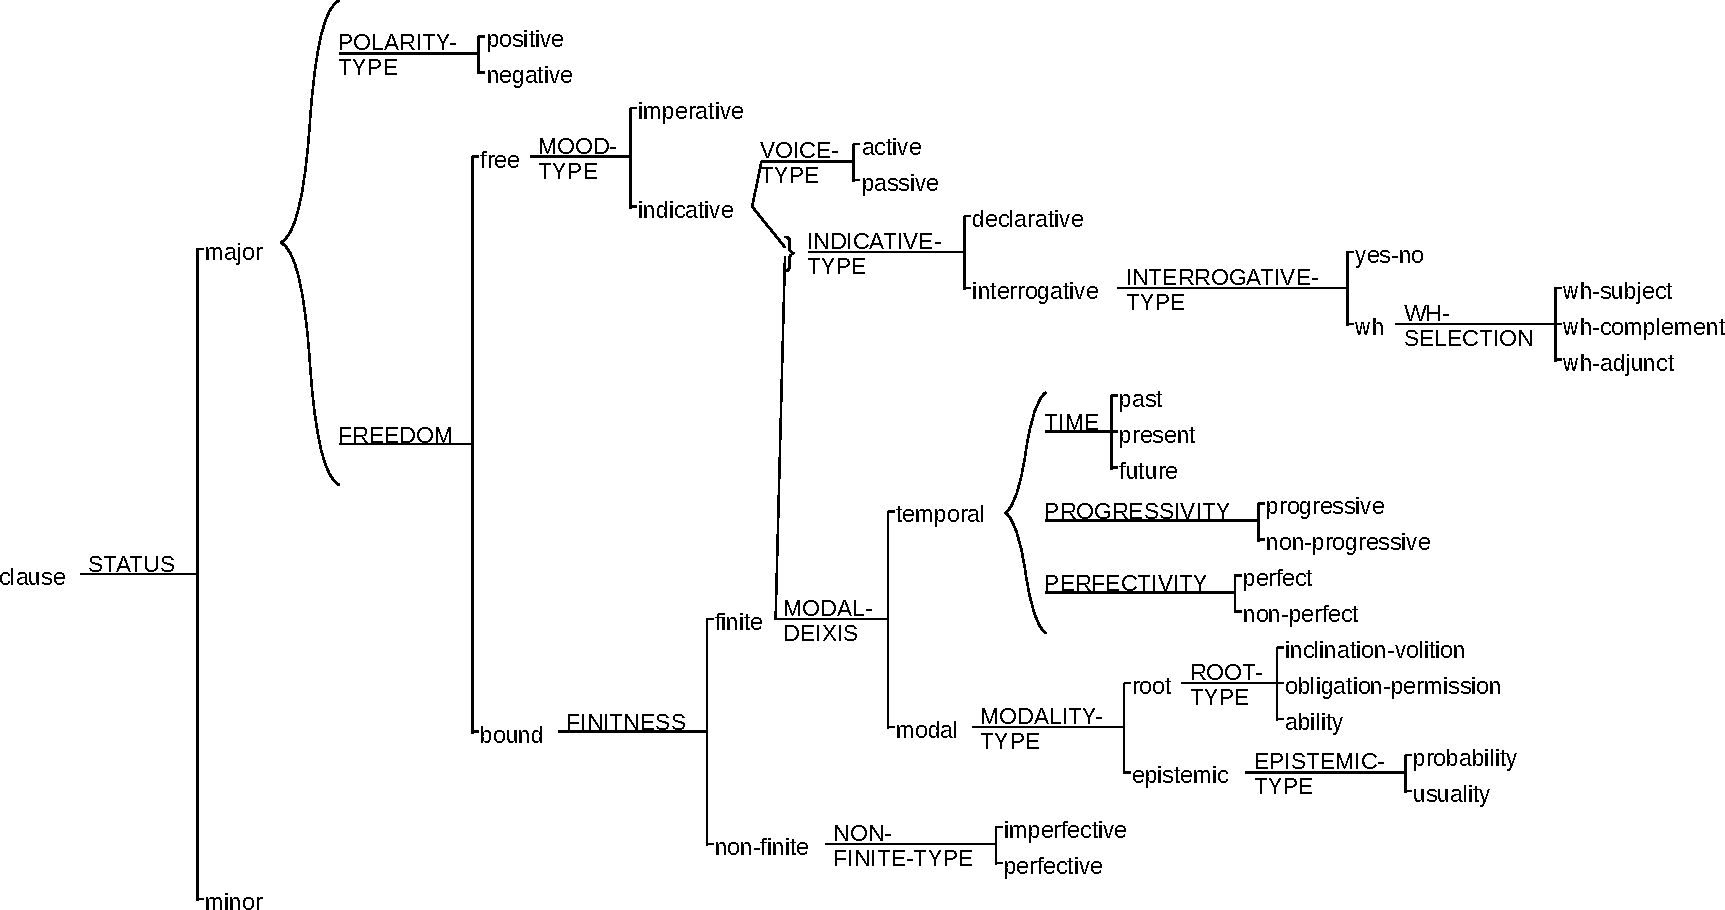
\includegraphics[width=\linewidth]{Figures/SFL-grammar/mood-simplified.pdf}
        \caption{An adaptation of the MOOD system network \citep[162]{Halliday2013}}
        \label{fig:clause-mood}
    \end{figure}

    The features of this feature network apply to units of clause class only. Even if some features may be intuitive I iterate briefly over each of them providing cues for identifying it. 
    
    The POLARITY system indicates whether the clause is affirmed or negated. The negative polarity is indicated, in English, by the presence of a clausal particle \textit{not} or \textit{n't}. It can also be signalled by similar negative markers in other clause elements such as the subject (e.g. ``None of the kids came to play.''), adjunct (e.g. ``He is never coming back.'') or complement (e.g. ``She loves no one.''). In the present work I consider the clausal negative marker only. 
    
    VOICE in traditional grammar indicates, for transitive verbs, whether the subject acts (\textit{active} voice) or is acted upon (\textit{passive} voice). In passive voice the subject and complement change position and the former is introduced by the preposition \textit{by}. 
    
    The semantics of the FREEDOM system is to indicate whether the clause is \textit{free} and realises a proposition or proposal and serves to develop an exchange in a dialogue either by initiating or responding to a speech act. On the other hand \textit{bound} clauses are not open to negotiation and serve as supporting information to be taken for granted. Structurally, the bound clauses usually depend on a dominant one that is free.
    
    The FINITENESS system indicates whether the clause is \textit{finite}, i.e. something that can be argued about. The way to make it arguable is by providing a point of reference into the here and now (\textit{temporal}) or into the speaker's judgement (\textit{modal}). The latter two features constitute the MODAL-DEIXIS system. 
    
    The MODALITY-TYPE system is an adaptation from \citet[689--692]{Halliday2013} that focuses on the usage of the modal verbs only and is organised into ROOT and EPISTEMIC modalities. The former one comprises \textit{inclination-volition}, \textit{obligation-permission} and \textit{ability} while the latter has \textit{usuality} and \textit{probability} features.
    
    The temporal feature indicates that the clause has a tense. For simplicity and ease the implementation into Parsimonious Vole, I replaced the Sydney account for tense with that of the traditional grammar of English. The systematisation is on three systems, that of TIME (past, present or future), PROGRESSIVITY (progressive or non-progressive) and PERFECTIVITY (perfect or non-perfect). The Sydney account for tense remains to be implemented in the future work.    
    
    In addition to the MOOD system network I include into the parsing process the DEIXIS system network for the nominal groups determination depicted in Figure \ref{fig:ng-determination}. The nominal DEIXIS system network is described in detail in IFG4 in the nominal group section \citep[364--396]{Halliday2013}. 
    
    \begin{figure}[!ht]
        \centering
        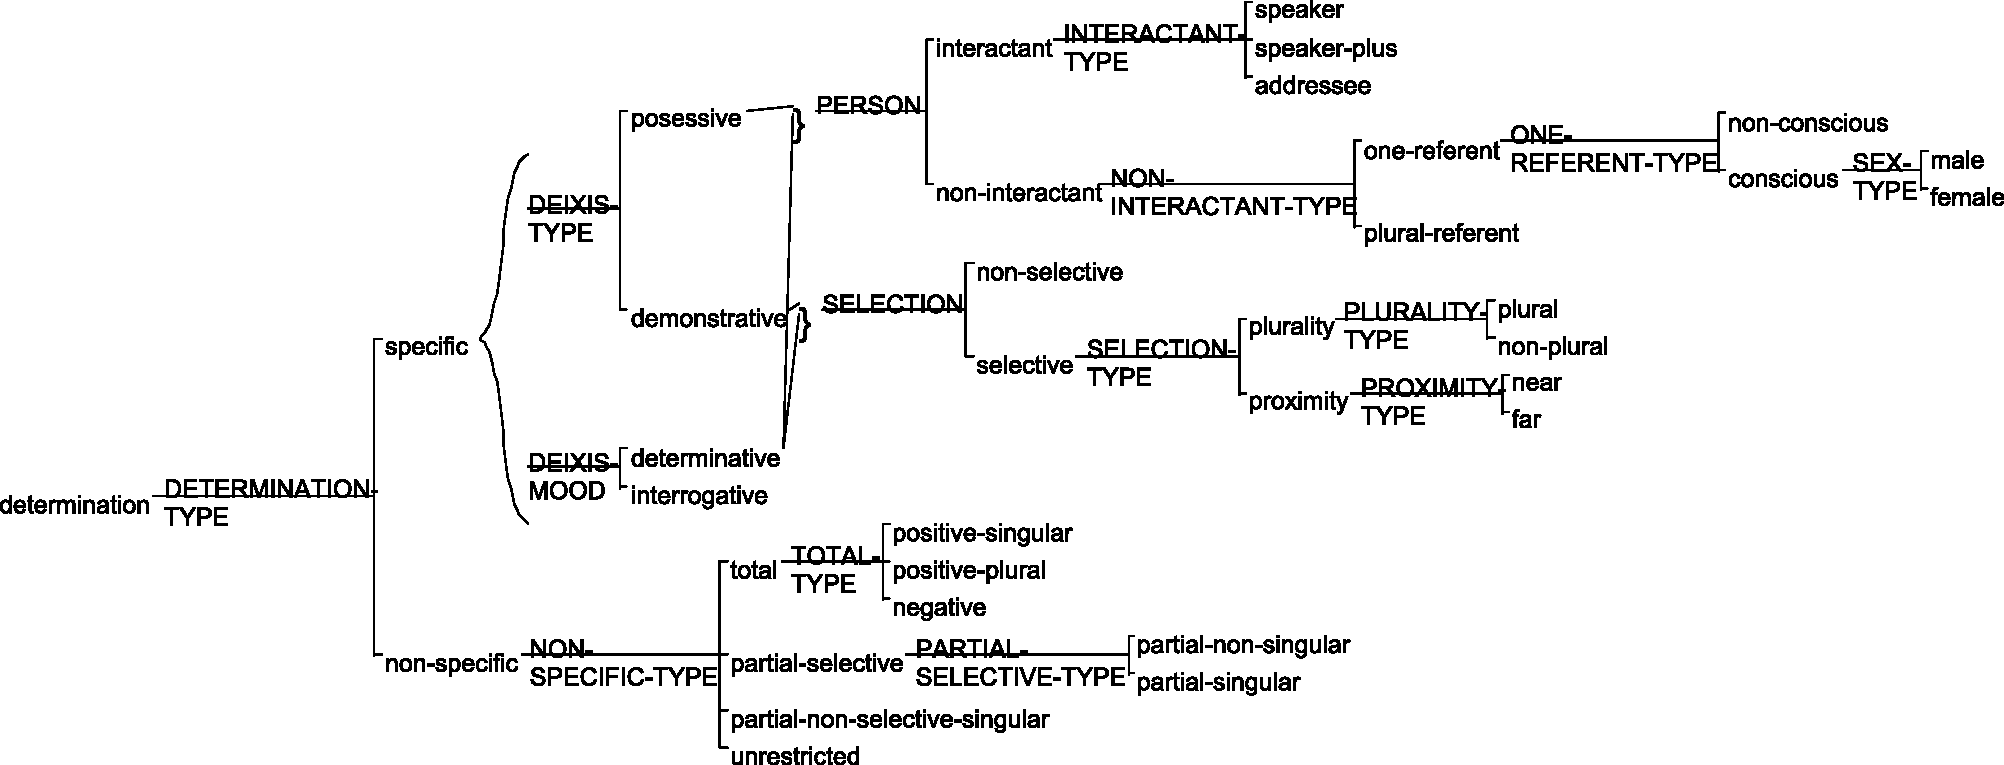
\includegraphics[width=\linewidth]{Figures/SFL-grammar/determination-system.pdf}
        \caption{The DEIXIS system network for nominal group determination \citep[366]{Halliday2013}}
        \label{fig:ng-determination}
    \end{figure}

    This system network is relevant for the current work because determining the systemic selections for the entire network can be unambiguously done based on lexical information only. In Section \ref{sec:enrichment-stage}, we will see a dictionary lookup method in addition to graph pattern matching to determine systemic selections. Next is briefly described the system network of TRANSITIVITY. 
      
\subsection{TRANSITIVITY}
\label{sec:transitivity}
    In Section \ref{sec:functions-metafunctions}, I explained that SFL organises the lexico-grammar in three parallel metafunctions. This section briefly recounts of the experiential metafunction and introduces the TRANSITIVITY system network that systematises it.
    
    In this perspective, ``the clause construes a quantum of change in a flow of events as a \textit{figure}, or a configuration of a \textit{process}, \textit{participants} involved in it and any attendant \textit{circumstance}'' \citep[212]{Halliday2013}. 
    
    In traditional grammar the term \textit{transitivity} refers to the property of verbs according to which they are classified into transitive and intransitive. In SFL the term transitivity is primarily concerned with clauses. It is most useful to refer to Halliday's TRANSITIVITY \citep{Halliday67-parts1+2,Halliday68-part3,Halliday68} that deals with Predicate, Subject, Complement, and Adjunct all of which are elements of the clause and are usually conflated with the Process, Participants and Circumstances. 

    The Sydney grammar makes a distinction between two types of experience: ``inner'' as experience inside ourselves and ``outer'' as experience in the world around us. The prototypical outer experience is that of actions and events. The inner experience is more difficult to sort but it is a kind of reply to the outer, recording it, reflecting on it, reacting to it etc. Two grammatical categories that realise these sort of experiences are the \textit{material} process and the \textit{mental} process.
    
    In addition to material and mental there is a third kind of process used in identifying, classifying and relating various kinds of experience. The grammatical category realising this type of link is the \textit{relational} process. Then using the combinations of the three main processes above, Halliday defines \textit{behavioural}, \textit{verbal} and \textit{existential} processes. 

    \begin{figure}[!ht]
        \centering
        \begin{tikzpicture}[]
        \node (re) [font=\bf] {realm of experience};
        \node (ph) [below=1em of re] {physical};
        \node (si) [below=1em of ph] {social interaction};
        \node (ps) [below=1em of si] {psychological};
        \node (ab) [below=1em of ps] {physical};
    
        \node (pt) [font=\bf, right=7em of re] {types of processes};
        \node (ac) [below=1em of pt] {action};
        \node (re) [below=1em of ac] {relational};
        \node (me) [below=1em of re] {mental};
        \node (in) [below=1em of me] {influential};        
        
        \draw [thick] (ph.east) -- (ac.west);
        \draw [thick] (ph.east) -- (re.west);
        \draw [thick] (ph.east) -- (in.west);
        
        \draw [thick] (si.east) -- (ac.west);
        \draw [thick] (si.east) -- (re.west);
        \draw [thick] (si.east) -- (in.west);
        
        \draw [thick] (ps.east) -- (me.west);
        \draw [thick] (ps.east) -- (re.west);
        \draw [thick] (ps.east) -- (in.west);
        
        \draw [thick] (ab.east) -- (re.west);
    
        \end{tikzpicture}
        \caption{The connections in Cardiff grammar between realms of experience and the process types}
        \label{fig:cardiff-realm-processtype}
    \end{figure}
    
    \begin{figure}[!ht]
        \centering
        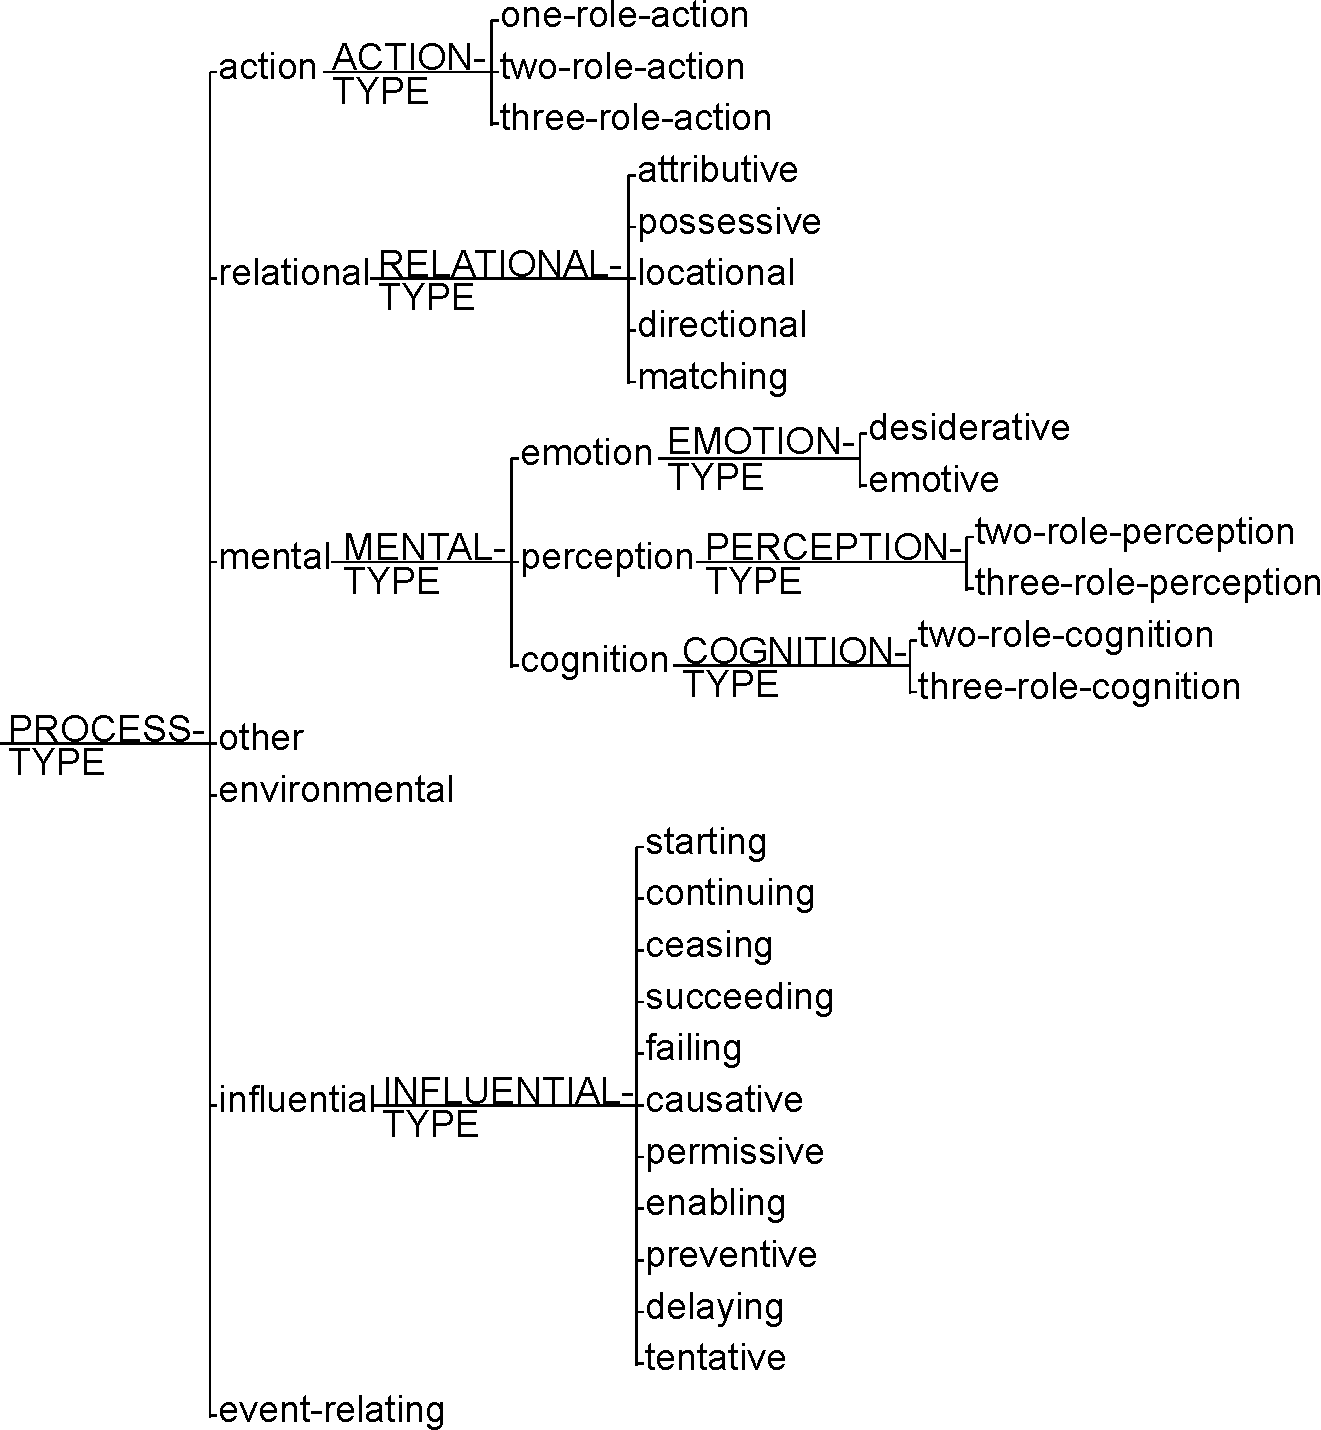
\includegraphics[width=0.8\linewidth]{Figures/SFL-grammar/Transitivity.pdf}
        \caption{Cardiff TRANSITIVITY system network}
        \label{fig:cardiff-transitivity}
    \end{figure}

    The Cardiff grammar employs similar process types, namely those of \textit{action}, \textit{relational}, \textit{mental} and \textit{influential}. In addition, it links these process types to realms of experience: \textit{physical}, \textit{social interaction}, \textit{psychological} and \textit{abstract}. Figure \ref{fig:cardiff-realm-processtype} provides the schematic connection between realms of experience and various process types that can realise that kind of experience \citep[37]{Fawcett2009}. 

    \citet{Fawcett1973,Fawcett87-relational,Fawcett96} has written the most on the TRANSITIVITY of the Cardiff grammar. It is a model that evolved over time and is depicted in Figure \ref{fig:cardiff-transitivity} in its latest form. The first main process type is the \textit{action}. It has been called ``material process'' in the past, but Fawcett returned to use the term ``action'' because there are many actions that are non-material, social for instance. The second main process is the \textit{relational} one, that is subdivided into \textit{attributive}, \textit{possessive}, \textit{locational}, \textit{directional} and \textit{matching}.

    The third main distinction is the \textit{mental} process that is divided into \textit{emotion}, \textit{perception} and \textit{cognition} distinctions. \textit{Environmental} processes, even if very rare, are recognised as another main process type. \textit{Influential} processes are unique to the Cardiff grammar and not accounted for elsewhere in the TRANSITIVITY system. The Cardiff grammar distinguishes the following influential processes: \textit{starting, ceasing, continuing, succeeding, failing, causative, permissive, enabling preventing, delaying and tentative}. These processes have a structural similarity, that of having an embedded event in the matrix process, which is somehow influenced. The last process type is that of \textit{event-relating} which is also a recent development specific to the Cardiff grammar. All the linguistic phenomena covered by this process are treated by Halliday as grammatical metaphors, but Fawcett considered they should be analysed as a distinct process type.
    
    The TRANSITIVITY system is highly dependent on the lexical semantics of the verbs. Therefore a broad account of verb senses and the participant configuration structures they command has to be provided in the grammar. \citet{Neale2002} has pioneered such work in her thesis, which I introduce in the next section. 

\subsection{Process Type Database}
\label{sec:ptdb-description-technical}

    The Process Type Database (PTDB) \citep{Neale2002} is the key resource in the automatic Transitivity analysis developed in this thesis and described in Chapter \ref{ch:enrichment-stage}. It is also the source for creating the graph patterns used to enrich the constituency graph as described in the same chapter. The PTDB provides information on what possible process types and participants can correspond to a particular verb meaning. The PTDB is a dictionary-like dataset of verbs bound to an exhaustive list of verb senses and the corresponding Process Configuration for each of them.
    
    In her work on PTDB \citet{Neale2002} improved the TRANSITIVITY system of the Cardiff Grammar by systematising over 5400 senses (and process configurations) for 2750 most common English verbs. Table \ref{tab:example-ptdb} presents a simplified sample of PTDB content.

    \begin{table}[!ht]
        \centering
        \resizebox{0.995\textwidth}{!}{%    
        \begin{tabulary}{1.2\textwidth}{|c|C|c|c|}
            \hline
            \textbf{verb form} & \textbf{informal meaning} & \textbf{process type} & \textbf{configuration} \\ \hline
            calculate & work out by mathematics (commission will then calculate the number of casted votes) & cognition & Ag-Cog + Ph \\ \hline
            & plan (newspaper articles were calculated to sway reader's opinions) & two role action & Ag + Cre \\ \hline
            catch & run after and seize (a leopard unable to catch its normal prey) & possessive & Ag-Ca + Af-Pos \\ \hline
            & fall ill (did you catch a cold?) & possessive & Ag-Ca + Af-Pos \\ \hline
            catch (up with) & reach (Simon tried to catch up with others) & two role action & Ag + Ra \\ \hline
        \end{tabulary}
        }
        \caption{An example of records in PTDB}
        \label{tab:example-ptdb}
    \end{table}

    The internal structure of the PTDB is detailed in Neale's PhD thesis \citep[193--231]{Neale2002}. In present thesis only three columns are of interest for the parsing purposes: the \textit{verb form} (1st), the Cardiff grammar \textit{process type} (6th) and the participant role \textit{configuration} (8th). The content of these columns is not uniform and so unsuitable for parsing purposes in its original form\footnote{see Neale's page  \url{http://www.itri.brighton.ac.uk/~Amy.Neale}}. The work on normalising and cleaning up the PTDB is described in Section \ref{sec:claning-ptdb}.


\section{Summary}
    This chapter has described the grammatical units and the two system networks adopted in this work. They constitute a selection from the Sydney and Cardiff grammars that are implemented in the Parsimonious Vole parser.
    
    Because of its bottom up approach to unit structure, rank scale relaxation and accommodation of embedding as a general principle, Cardiff systemic functional theory is more suitable for parsing than the Sydney one. Nonetheless the unit definitions in the Cardiff grammar are deeply semantic in nature. Parsing with such units requires most of the time lexical-semantically informed decisions beyond merely syntactic variations. This is one of the reasons why the parsing attempts by \citet{ODonoghue1991a} and others in the COMMUNAL project were all based on a corpus (which is not available to the current work). 
    
    In the present thesis the syntagmatic structures are built based on transformations from the Stanford Dependency grammar motivated in the first chapter. Stanford dependency relations are closely related to the traditional grammar just like the Penn part of speech tag set, which is integrated into the dependency graphs produced by the Stanford parser. This is the reason to adapt in this thesis Sydney unit structures as they are closer to traditional grammar syntax \citep{Quirk1985}, which makes the parsing task easier.
    
    The next chapter lays the theoretical foundations of Dependency Grammar and introduces the Stanford dependency parser, which is used as a departing point in the current parsing pipeline (see Section \ref{sec:architecture}). Because there is a transformation step from dependency to systemic functional consistency structure, the next chapter also covers a theoretical compatibility analysis and how such a transformation should in principle look. 

